\chapter{ANEXOS}
\begin{landscape}
\begin{table}[ht]
\centering
\caption{MAPIC}
\label{tab:mapic}
\begin{tabular}{|l|l|l|}
\hline
%\rowcolor[HTML]{C0C0C0} 
\textbf{VARIABLE FÁCTICA}            & \textbf{DIMENSIONES}                    & \textbf{INDICADORES}                           \\ \hline
Diseño de itinerario personalizado   & Tiempo                                  & Días                                           \\ \hline
                                     &                                         & Horas                                          \\ \hline
                                     &                                         & Minutos                                        \\ \hline
                                     & Costo                                   & Soles                                          \\ \hline
                                     &                                         & Dólares                                        \\ \hline
                                     & Distancias                              & Km.                                            \\ \hline
                                     &                                         & Metros                                         \\ \hline
                                     & Valoración de la actividad              & Puntaje(relevancia) de la actividad            \\ \hline
                                     &                                         & Preferencia del turista por tipo de actividad  \\ \hline
%\rowcolor[HTML]{C0C0C0} 
\textbf{VARIABLE TEMÁTICA}           & \textbf{EJES TEMÁTICOS}                 & \textbf{SUBEJES TEMÁTICOS}                     \\ \hline
+Optimización combinatoria           & ~Optimización multiobjetivo             & Formulación del modelo matemático              \\ \hline
                                     &                                         & Solución del modelo                            \\ \hline
                                     &                                         & Evaluación del modelo                          \\ \hline
                                     &                                         & Validación del modelo                          \\ \hline
                                     &                                         & Implementación                                 \\ \hline
Meteheurística                       & Heurística de construcción              & Vecino mas Cercano                             \\ \hline
                                     & Heurística de mejoría                   & 2-opt                                          \\ \hline
                                     & Metaheurística                          & Búsqueda Tabú                                  \\ \hline
%\rowcolor[HTML]{C0C0C0} 
\textbf{VARIABLE PROPOSITIVA}        & \textbf{EJES PROPOSITIVOS}              & \textbf{SUBEJES PROPOSITIVOS}                  \\ \hline
Implementación de modelo inteligente & Implementación de la solución del modelo & Codificación de la heurística de construcción \\ \hline
                                     &                                         & Codificación heurística de mejoría             \\ \hline
                                     &                                         & Codificación de la metaheurística              \\ \hline
                                     & Validación                              & Validación con instancias reales               \\ \hline
                                     &                                         & Validación con instancias artificiales         \\ \hline
                                     & Implementación en un módulo             & Codificación del backend                       \\ \hline
                                     &                                         & Codificacion del frontend                      \\ \hline
\end{tabular}
\end{table}
\end{landscape}

\section{Perfil del Turista Extranjero que visita Puno - 2017}
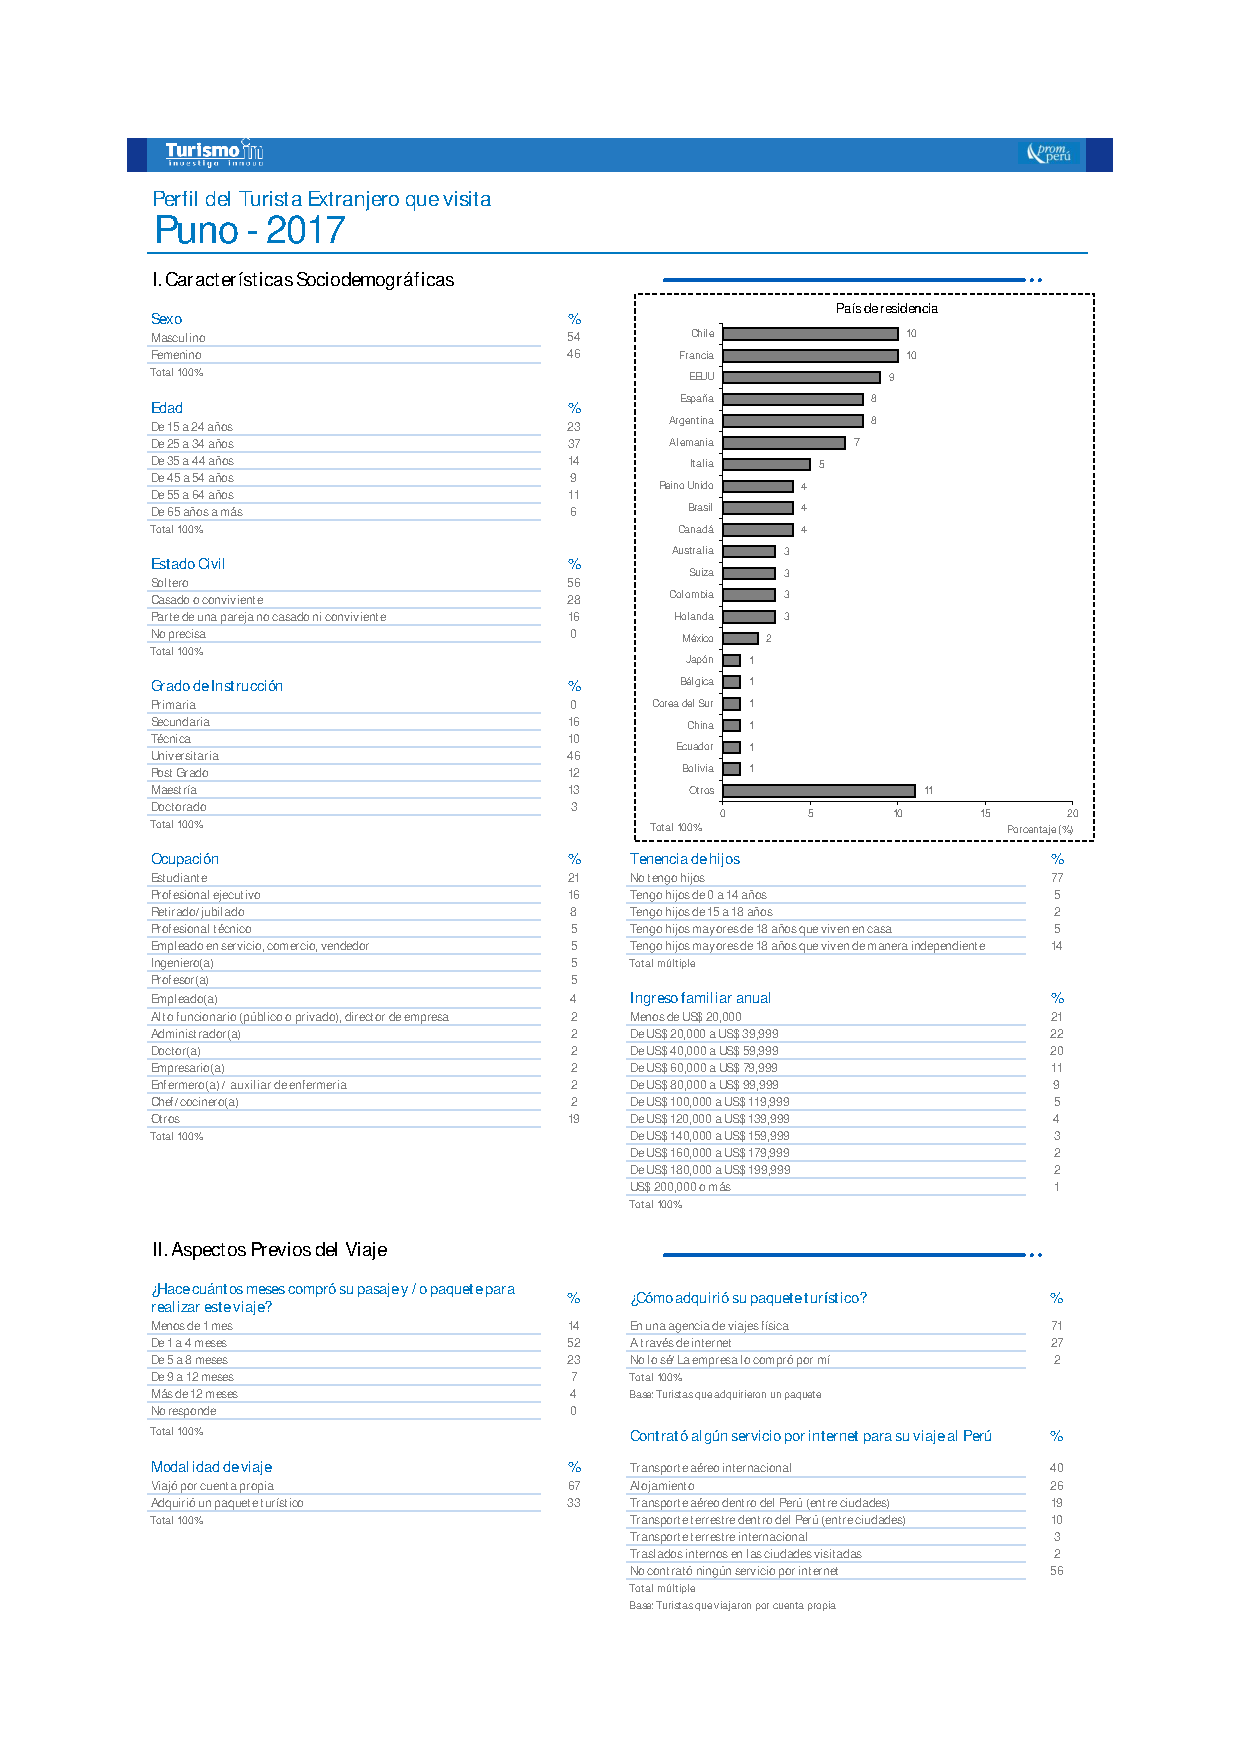
\includepdf[pages=-]{Capitulo7/files/2017-Perfil_del_Turista_Extranjero_que_visita_Puno_-_2017.pdf}
%\includepdf[pages=-, scale=0.9]{p01.pdf}
